\section{Filtros de preservación de bordes}

    El filtro gaussiano reduce el ruido promediando cada píxel con sus vecinos según la distancia, sin distinguir si esos vecinos pertenecen al mismo objeto, por lo que también suaviza los bordes. El filtro bilateral agrega un segundo peso que depende de la diferencia de intensidad, de modo que sólo promedia vecinos cercanos \textbf{y} parecidos. El objetivo de esta actividad es comparar el desempeño de ambos filtros analizándolos sobre una imagen limpia la cual fue contaminada con ruido gaussiano moderado ($\sigma \approx 20$--$25$), para esto se variaron los parámetros de manera visual y cuantitativamente, en regiones de borde y  homogéneas, eligiendo la configuración más adecuada priorizando las métricas SSIM (\textit{Structural Similarity Index Measure} o Índice de Similitud Estructural) y PSNR (\textit{Peak Signal-to-Noise Ratio} o Relación Señal a Ruido de Pico).

    Se usó una fotografía de una disquería tomada con un celular, de $6120\times6120$ píxeles en color. La escena combina zonas homogéneas (la pared), bordes muy marcados (las guitarras colgadas contra la pared) y detalle fino (lomos de discos y estanterías). Se redujo a $1024\times1024$ con interpolación por área (\texttt{INTER\_AREA}), que promedia bloques de unos $6\times6$ píxeles. Esto atenúa el ruido propio del sensor, tomado con poca luz, deja una referencia limpia (\textit{ground truth}) y vuelve viable el barrido de parámetros, ya que el bilateral sobre 37 megapíxeles tarda segundos por configuración. Todo se implementó en Python con OpenCV (\textit{Open Source Computer Vision Library} o Biblioteca de Visión por Computadora de Código Abierto) y scikit-image.

    \subsection{Imagen de referencia y contaminación}

        Se sumó ruido gaussiano aditivo $n \sim \mathcal{N}(0, 25^2)$, independiente en cada píxel y canal, con semilla fija para que sea reproducible, y se recortó el resultado a $[0, 255]$ (\textbf{Figura \ref{fig:ej2_ruido}}). Sobre la referencia se definieron dos ROI (\textit{Region of Interest} o Región de Interés), recortes de la imagen elegidos para analizarlos de cerca. Una es de \textbf{borde}, con las guitarras contra la pared, y la otra es \textbf{homogénea}, con la pared lisa. También se trazó una línea de perfil que cruza las guitarras.

        \begin{figure}[H] \centering
            \begin{subfigure}[b]{0.31\linewidth} \centering
                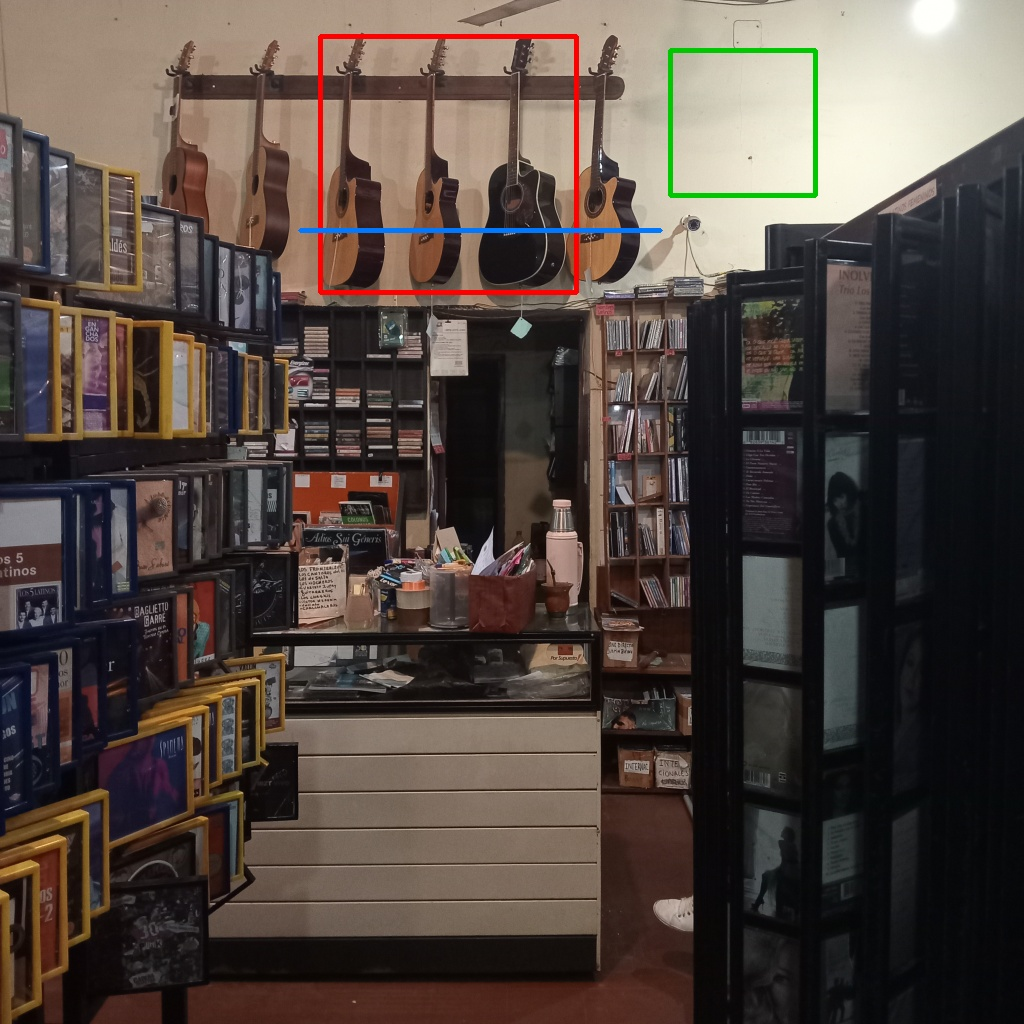
\includegraphics[width=\linewidth]{img/ejercicio_2/original_rois.jpg}
                \caption{Referencia}
            \end{subfigure}
            \hspace{0.04\linewidth}
            \begin{subfigure}[b]{0.31\linewidth} \centering
                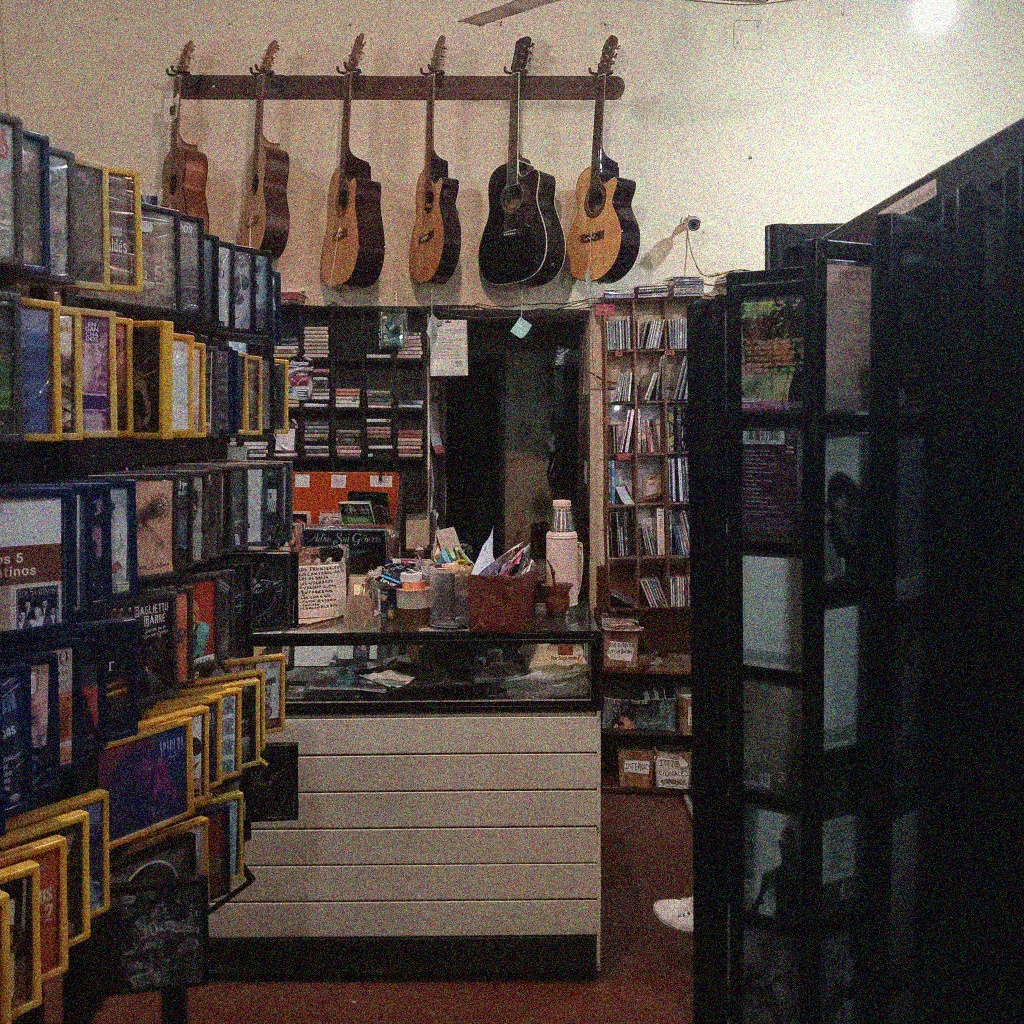
\includegraphics[width=\linewidth]{img/ejercicio_2/ruidosa_gauss25.jpg}
                \caption{Ruido gaussiano $\sigma=25$}
            \end{subfigure}
            \caption{Referencia con las ROI de borde (rojo), homogénea (verde) y perfil (azul).}
            \label{fig:ej2_ruido}
        \end{figure}

    \subsection{Filtros y métricas}

        El \textbf{filtro gaussiano} pondera cada vecino $q$ del píxel $p$ sólo por su distancia, con $G_\sigma(x) = e^{-x^2/2\sigma^2}$. El \textbf{filtro bilateral} \cite{ej2:tomasi} multiplica ese peso espacial por un peso de rango, que depende de la diferencia de intensidad $|I_p - I_q|$,
        \begin{equation*}
            BF(p) = \frac{1}{W_p}\sum_{q} G_{\sigma_{esp}}\!\left(\lVert p-q \rVert\right)\, G_{\sigma_{rango}}\!\left(|I_p - I_q|\right)\, I_q ,
            \qquad W_p = \sum_{q} G_{\sigma_{esp}}\, G_{\sigma_{rango}} .
        \end{equation*}
        donde $BF(p)$ es la salida del filtro bilateral (\textit{Bilateral Filter} o Filtro Bilateral) en $p$, $I_q$ la intensidad del vecino $q$ y $W_p$ la suma de los pesos, que normaliza el resultado.

        Se probó el gaussiano con $\sigma_{esp} \in \{2, 4, 6\}$ y el bilateral con todas las combinaciones de $\sigma_{esp} \in \{2, 4, 6\}$ y $\sigma_{rango} \in \{20, 50, 100\}$, dando doce configuraciones en total. OpenCV fija la ventana del gaussiano en $6\sigma+1$ píxeles (13, 25 y 37 para nuestro caso). La del bilateral (con \texttt{d=0}) la obtiene de un radio de $1{,}5\,\sigma_{esp}$ (7, 13 y 19). En imágenes a color, OpenCV mide la diferencia de rango como la \textbf{suma de las diferencias absolutas de los tres canales} \cite{ej2:opencv}, lo que condiciona la escala de $\sigma_{rango}$.

        Cada resultado se comparó con la referencia mediante el MSE (\textit{Mean Squared Error} o Error Cuadrático Medio), el PSNR y el SSIM, descritos en la \textbf{Tabla \ref{tab:ej2_metricas}}, sobre los tres canales y con rango dinámico fijo de 255. El tiempo se midió con 7 repeticiones de 3 ejecuciones y se reporta la mediana, robusta ante interrupciones del sistema.

        \begin{table}[H] \centering \setstretch{1.05} \captionsetup{labelfont=bf}
            \begin{tblr}{
                cells={valign=m, halign=l, font=\small}, colspec={Q[2.2cm] Q[4.6cm] X[l]},
                rowsep=1.5pt, colsep=4pt, hlines, vlines,
                row{1}={bg=gray!15, font=\small\bfseries, halign=c}, column{1}={halign=c} }
                Métrica & Cómo se calcula & Qué mide y para qué se usa \\
                MSE $\downarrow$ & $\frac{1}{N}\sum (x-y)^2$, en niveles de gris$^2$ & Error cuadrático medio píxel a píxel. Vale 0 si son idénticas y no considera la percepción. \\
                PSNR $\uparrow$ \cite{ej2:gonzalez} & $10\log_{10}\!\left(255^2/\mathrm{MSE}\right)$ [dB] & Relación entre el valor máximo y el error. Más de 30 dB se considera bueno, aunque hereda las limitaciones del MSE. \\
                SSIM $\uparrow$ \cite{ej2:wang} & Producto de luminancia, contraste y estructura en ventanas locales & Similitud estructural, de 0 a 1. Detecta bordes borroneados y texturas perdidas, y su mapa local muestra \textit{dónde} falla. \\
                Puesto promedio $\downarrow$ & Promedio de los puestos en SSIM y en PSNR & Criterio de decisión que combina estructura y fidelidad. Si hay empate, decide el SSIM. \\
            \end{tblr}
            \caption{Métricas de calidad usadas, donde $\uparrow$ indica que conviene un valor mayor y $\downarrow$, uno menor.}
            \label{tab:ej2_metricas}
        \end{table}

    \subsection{Resultados globales}

        La \textbf{Tabla \ref{tab:ej2_resultados}} resume las doce configuraciones ordenadas por puesto promedio, y la \textbf{Figura \ref{fig:ej2_curvas}} muestra cómo varían SSIM y PSNR con $\sigma_{rango}$.

        \begin{itemize}[label=\textbullet]
            \item \textbf{Con $\sigma_{rango}=20$ el bilateral casi no filtra}. El SSIM apenas pasa de 0,302 a valores de entre 0,326 y 0,357. Con $\sigma=25$ por canal, dos vecinos de una misma zona difieren en promedio unos 85 niveles en la suma de los tres canales, muy por encima de 20.
            \item \textbf{Con $\sigma_{rango}=100$ el bilateral supera a todos los gaussianos} en ambas métricas. La configuración $(4, 100)$ logra un SSIM de 0,814 y un PSNR de 29,84 dB, contra 0,769 y 26,30 dB del mejor gaussiano ($\sigma=2$).
            \item \textbf{El gaussiano empeora al aumentar $\sigma$}. Con $\sigma=6$ el PSNR cae a 22,70 dB. A esa escala, el error por borronear los bordes supera lo que se gana al quitar ruido.
            \item \textbf{PSNR y SSIM no eligen lo mismo}. La configuración $(2, 100)$ tiene el menor MSE y el mayor PSNR (29,92 dB) porque conserva mejor los bordes, pero en las zonas lisas deja más ruido residual (\textbf{Figura \ref{fig:ej2_grano}}) y su SSIM baja a 0,761. El ruido residual es el desvío estándar de la diferencia entre la imagen filtrada y la referencia en los píxeles homogéneos, y vale 6,2 niveles de intensidad (escala de 0 a 255) con $(2, 100)$, 4,6 con $(4, 100)$ y 22,2 en la imagen ruidosa. Priorizar el SSIM implica aumentar $\sigma_{esp}$ de 2 a 4, con lo que se elige $(4, 100)$.
        \end{itemize}

        \begin{table}[H] \centering \setstretch{1.05} \captionsetup{labelfont=bf}
            \begin{tblr}{
                cells={valign=m, halign=c, font=\small}, colspec={Q Q Q Q Q Q Q Q},
                rowsep=0.8pt, colsep=5pt, hlines, vlines,
                row{1}={bg=gray!15, font=\small\bfseries},
                row{2}={font=\small\bfseries},
                cell{2}{6}={bg=gray!25}, cell{4}{4}={bg=gray!25}, cell{4}{5}={bg=gray!25},
                cell{5}{7}={bg=gray!25}, cell{2}{8}={bg=gray!25} }
                Filtro & $\sigma_{esp}$ & $\sigma_{rango}$ & MSE $\downarrow$ & PSNR $\uparrow$ & SSIM $\uparrow$ & Tiempo [ms] $\downarrow$ & Puesto $\downarrow$ \\
                Bilateral & 4 & 100 & 67,5  & 29,84 & 0,814 & 67,0 & 1,5 \\
                Bilateral & 6 & 100 & 80,9  & 29,05 & 0,802 & 153,5 & 2,5 \\
                Bilateral & 2 & 100 & 66,3  & 29,92 & 0,761 & 19,6 & 2,5 \\
                Gaussiano & 2 & --  & 152,3 & 26,30 & 0,769 & 4,8 & 4,5 \\
                Bilateral & 6 & 50  & 109,2 & 27,75 & 0,624 & 149,7 & 5,5 \\
                Gaussiano & 4 & --  & 256,6 & 24,04 & 0,696 & 14,2 & 6,5 \\
                Bilateral & 4 & 50  & 112,5 & 27,62 & 0,618 & 67,6 & 6,5 \\
                Gaussiano & 6 & --  & 348,8 & 22,70 & 0,646 & 17,3 & 7,5 \\
                Bilateral & 2 & 50  & 153,9 & 26,26 & 0,548 & 17,2 & 8,0 \\
                Bilateral & 6 & 20  & 376,1 & 22,38 & 0,357 & 152,4 & 10,0 \\
                Bilateral & 4 & 20  & 402,3 & 22,09 & 0,347 & 61,2 & 11,0 \\
                Bilateral & 2 & 20  & 458,4 & 21,52 & 0,326 & 17,1 & 12,0 \\
                Ruidosa   & -- & -- & 527,4 & 20,91 & 0,302 & -- & -- \\
            \end{tblr}
            \caption{Métricas de las doce configuraciones, con el mejor valor en gris y la elegida en negrita.}
            \label{tab:ej2_resultados}
        \end{table}

        \begin{figure}[H] \centering
            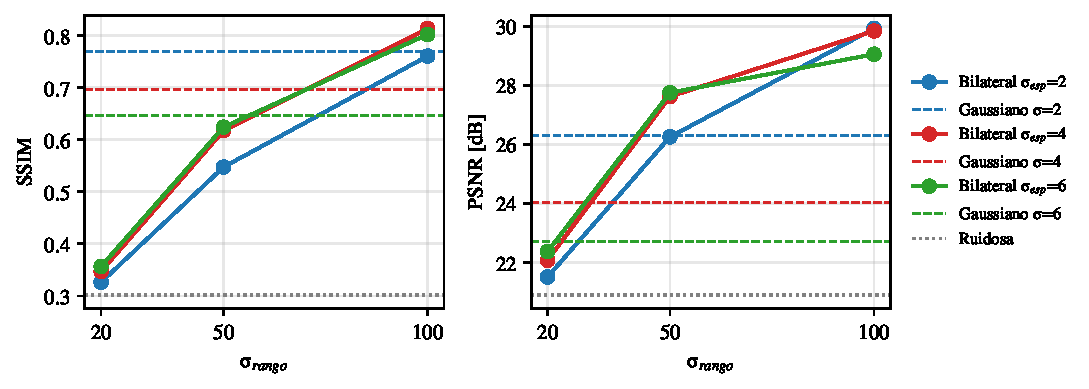
\includegraphics[width=0.82\linewidth]{img/ejercicio_2/curvas_metricas.pdf}
            \caption{SSIM y PSNR del bilateral según $\sigma_{rango}$, con el gaussiano de igual $\sigma$ en punteado.}
            \label{fig:ej2_curvas}
        \end{figure}

        \begin{figure}[H] \centering
            \begin{subfigure}[t]{0.2\linewidth}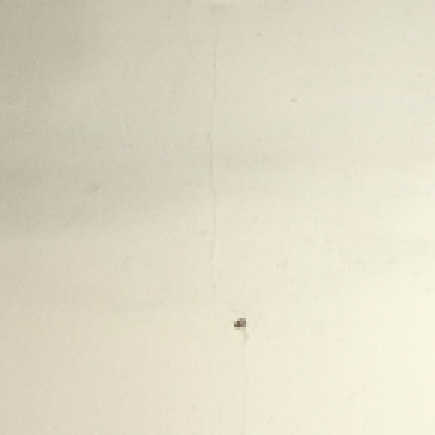
\includegraphics[width=\linewidth]{img/ejercicio_2/roi_homog_original.png}\caption{Referencia}\end{subfigure}\hspace{0.02\linewidth}
            \begin{subfigure}[t]{0.2\linewidth}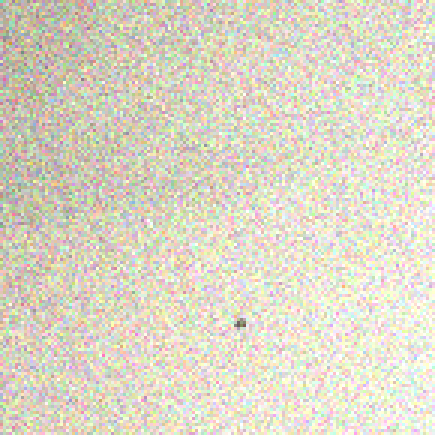
\includegraphics[width=\linewidth]{img/ejercicio_2/roi_homog_ruidosa.png}\caption{Ruidosa}\end{subfigure}\hspace{0.02\linewidth}
            \begin{subfigure}[t]{0.2\linewidth}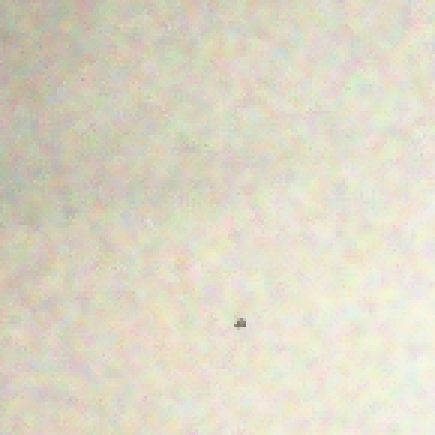
\includegraphics[width=\linewidth]{img/ejercicio_2/roi_homog_bil_s2_r100.png}\caption{Bilateral $(2, 100)$}\end{subfigure}\hspace{0.02\linewidth}
            \begin{subfigure}[t]{0.2\linewidth}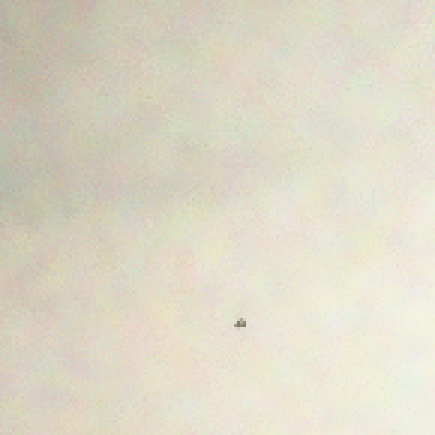
\includegraphics[width=\linewidth]{img/ejercicio_2/roi_homog_bil_s4_r100.png}\caption{Bilateral $(4, 100)$}\end{subfigure}
            \caption{Ruido residual de $(2, 100)$ y de $(4, 100)$ en la ROI homogénea.}
            \label{fig:ej2_grano}
        \end{figure}

    \subsection{Regiones de borde y homogéneas}

        El desempeño de ambos filtros en regiones de borde y homogéneas se evaluó con dos enfoques. Primero se midieron las métricas dentro de las dos ROI, y después, para salvar las limitaciones de ese enfoque, sobre máscaras que clasifican todos los píxeles de la imagen. En los dos se fijó $\sigma_{esp}=4$, para analizar ambos filtros a la misma escala espacial, y se varió $\sigma_{rango}$ (\textbf{Figura \ref{fig:ej2_rois}}).

        \begin{figure}[H] \centering
            \begin{subfigure}[b]{0.158\linewidth}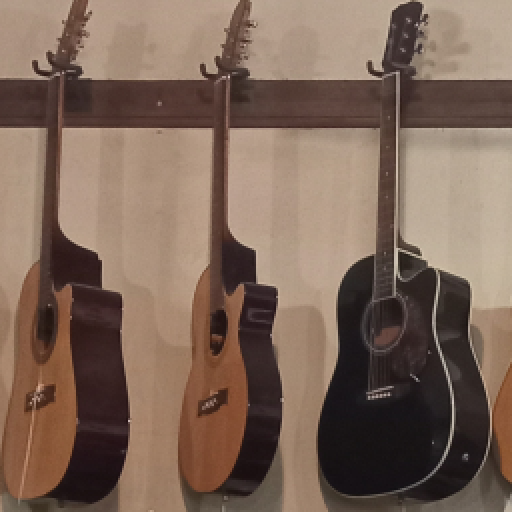
\includegraphics[width=\linewidth]{img/ejercicio_2/roi_borde_original.png}\end{subfigure}\hfill
            \begin{subfigure}[b]{0.158\linewidth}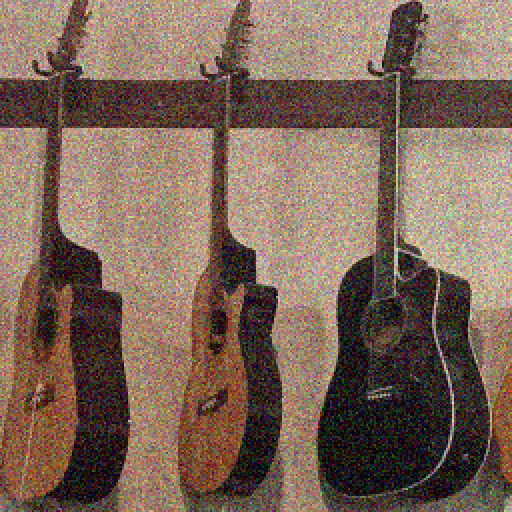
\includegraphics[width=\linewidth]{img/ejercicio_2/roi_borde_ruidosa.png}\end{subfigure}\hfill
            \begin{subfigure}[b]{0.158\linewidth}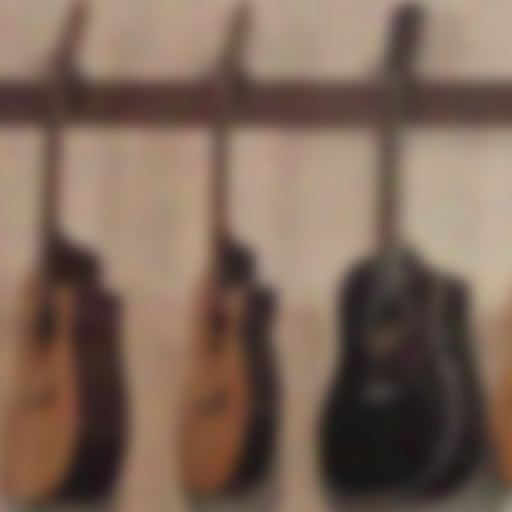
\includegraphics[width=\linewidth]{img/ejercicio_2/roi_borde_gauss_s4.png}\end{subfigure}\hfill
            \begin{subfigure}[b]{0.158\linewidth}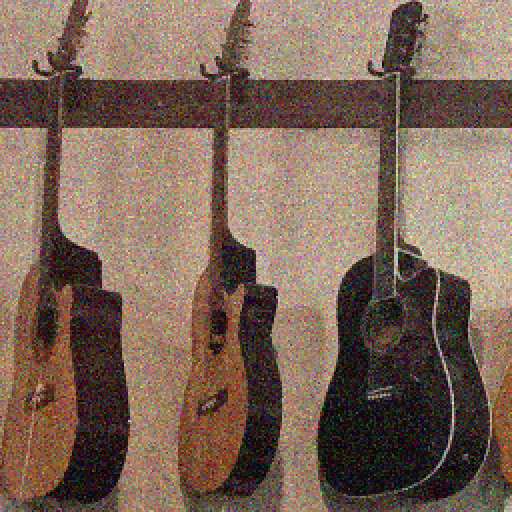
\includegraphics[width=\linewidth]{img/ejercicio_2/roi_borde_bil_s4_r20.png}\end{subfigure}\hfill
            \begin{subfigure}[b]{0.158\linewidth}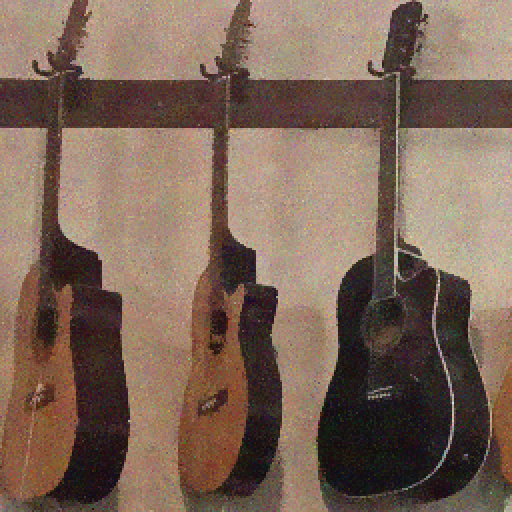
\includegraphics[width=\linewidth]{img/ejercicio_2/roi_borde_bil_s4_r50.png}\end{subfigure}\hfill
            \begin{subfigure}[b]{0.158\linewidth}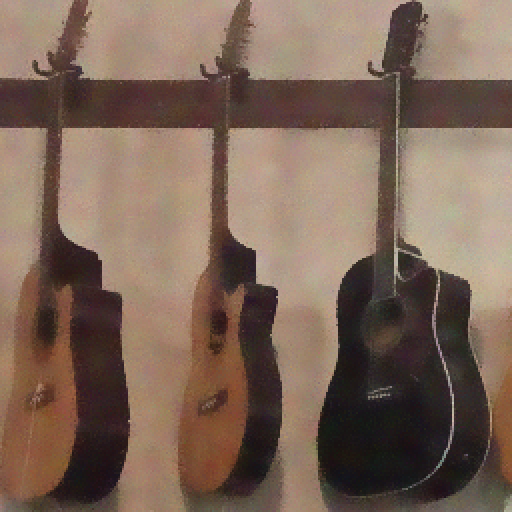
\includegraphics[width=\linewidth]{img/ejercicio_2/roi_borde_bil_s4_r100.png}\end{subfigure}
            \par\vspace{0.1cm}
            \begin{subfigure}[t]{0.158\linewidth}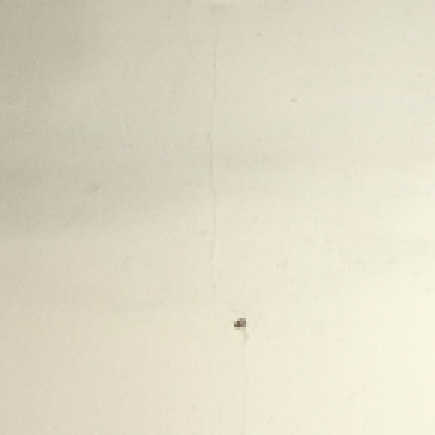
\includegraphics[width=\linewidth]{img/ejercicio_2/roi_homog_original.png}\caption{Referencia}\end{subfigure}\hfill
            \begin{subfigure}[t]{0.158\linewidth}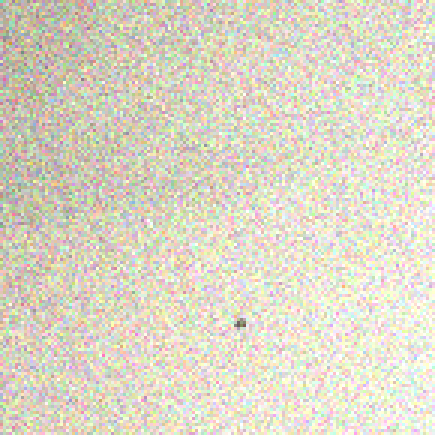
\includegraphics[width=\linewidth]{img/ejercicio_2/roi_homog_ruidosa.png}\caption{Ruidosa}\end{subfigure}\hfill
            \begin{subfigure}[t]{0.158\linewidth}
\includegraphics[width=\linewidth]{img/ejercicio_2/roi_homog_gauss_s4.png}\caption{Gaussiano}\end{subfigure}\hfill
            \begin{subfigure}[t]{0.158\linewidth}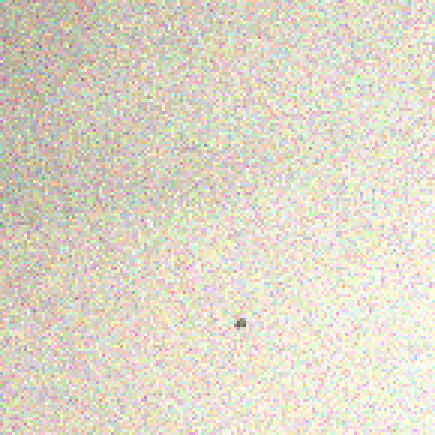
\includegraphics[width=\linewidth]{img/ejercicio_2/roi_homog_bil_s4_r20.png}\caption{Bil. $\sigma_{r}{=}20$}\end{subfigure}\hfill
            \begin{subfigure}[t]{0.158\linewidth}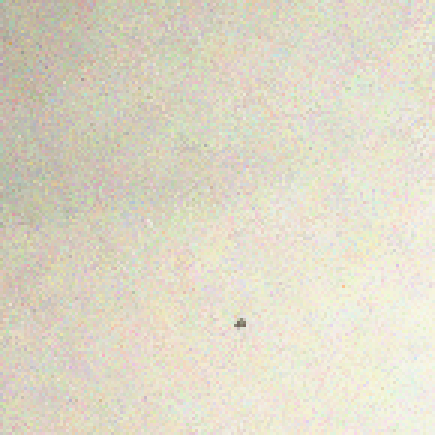
\includegraphics[width=\linewidth]{img/ejercicio_2/roi_homog_bil_s4_r50.png}\caption{Bil. $\sigma_{r}{=}50$}\end{subfigure}\hfill
            \begin{subfigure}[t]{0.158\linewidth}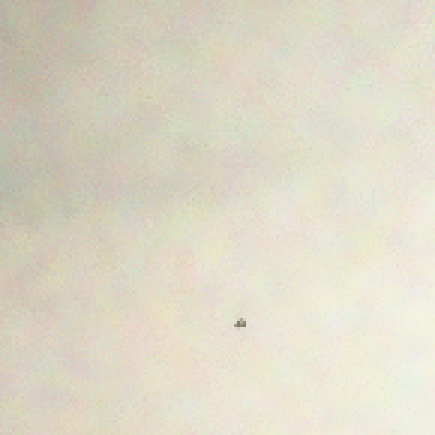
\includegraphics[width=\linewidth]{img/ejercicio_2/roi_homog_bil_s4_r100.png}\caption{Bil. $\sigma_{r}{=}100$}\end{subfigure}
            \caption{ROI de borde (arriba) y homogénea (abajo) con $\sigma_{esp}=4$ en ambos filtros.}
            \label{fig:ej2_rois}
        \end{figure}

        En el primer enfoque, el PSNR y el SSIM se calcularon sólo con los píxeles de cada recorte, comparando la referencia con la imagen filtrada completa y luego recortada (\textbf{Tablas \ref{tab:ej2_roi_borde} y \ref{tab:ej2_roi_homog}}).

        \begin{table}[H] \centering \setstretch{1.05} \captionsetup{labelfont=bf}
            \begin{minipage}[t]{0.48\linewidth} \centering
                \begin{tblr}{
                    cells={valign=m, halign=c, font=\small}, colspec={Q[l] Q Q},
                    rowsep=0.8pt, colsep=5pt, hlines, vlines,
                    row{1}={bg=gray!15, font=\small\bfseries},
                    cell{5}{2}={bg=gray!25}, cell{5}{3}={bg=gray!25} }
                    Imagen & PSNR [dB] $\uparrow$ & SSIM $\uparrow$ \\
                    Ruidosa & 20,37 & 0,322 \\
                    Gaussiano $\sigma=2$ & 25,75 & 0,754 \\
                    Gaussiano $\sigma=4$ & 23,21 & 0,658 \\
                    Bilateral $(4, 100)$ & 30,49 & 0,814 \\
                \end{tblr}
                \caption{Métricas en la ROI de borde.}
                \label{tab:ej2_roi_borde}
            \end{minipage}\hfill
            \begin{minipage}[t]{0.48\linewidth} \centering
                \begin{tblr}{
                    cells={valign=m, halign=c, font=\small}, colspec={Q[l] Q Q},
                    rowsep=0.8pt, colsep=5pt, hlines, vlines,
                    row{1}={bg=gray!15, font=\small\bfseries},
                    cell{4}{2}={bg=gray!25}, cell{4}{3}={bg=gray!25} }
                    Imagen & PSNR [dB] $\uparrow$ & SSIM $\uparrow$ \\
                    Ruidosa & 20,77 & 0,112 \\
                    Gaussiano $\sigma=2$ & 35,20 & 0,894 \\
                    Gaussiano $\sigma=4$ & 36,88 & 0,961 \\
                    Bilateral $(4, 100)$ & 35,22 & 0,843 \\
                \end{tblr}
                \caption{Métricas en la ROI homogénea.}
                \label{tab:ej2_roi_homog}
            \end{minipage}
        \end{table}

        En la ROI de borde, el bilateral $(4, 100)$ obtiene el mejor PSNR (30,49 dB) y el mejor SSIM (0,814), contra 23,21 dB y 0,658 del gaussiano $\sigma=4$, que borronea el contorno de las guitarras (\textbf{Figura \ref{fig:ej2_rois}}, fila superior). El perfil de la \textbf{Figura \ref{fig:ej2_perfil}}, tomado sobre la línea azul de la \textbf{Figura \ref{fig:ej2_ruido}}, muestra que el gaussiano convierte cada escalón guitarra--pared en una rampa de unos 15 píxeles y aplana los picos finos, como las cuerdas. El bilateral sigue a la referencia y sólo elimina la oscilación del ruido, aunque se aprecia visualmente que mayores valores de $\sigma_{r}$ difuminan más los bordes.

        En la ROI homogénea el orden se invierte. El gaussiano $\sigma=4$ deja la pared más lisa (SSIM 0,961 contra 0,843 del bilateral), porque el bilateral conserva un grano leve (\textbf{Figura \ref{fig:ej2_rois}}, fila inferior), aunque los tres filtros superan los 35 dB de PSNR.

        \begin{figure}[H] \centering
            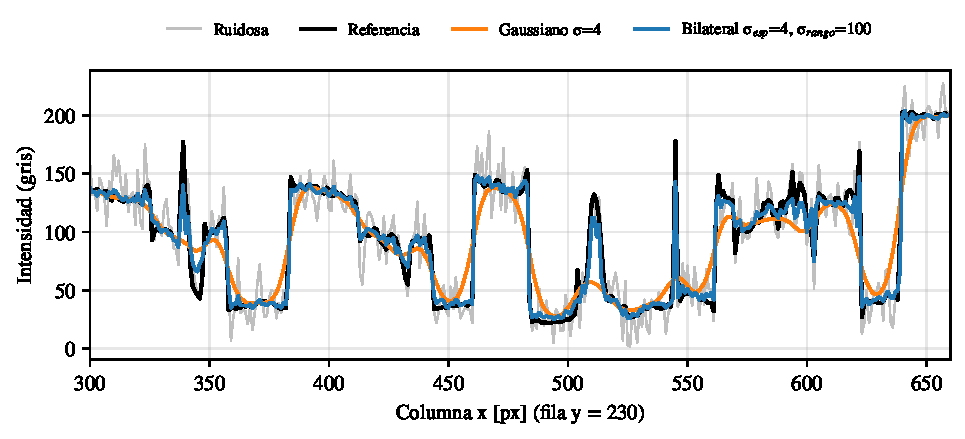
\includegraphics[width=0.8\linewidth]{img/ejercicio_2/perfil_borde.pdf}
            \caption{Perfil de intensidad sobre la fila 230, que atraviesa cuatro guitarras.}
            \label{fig:ej2_perfil}
        \end{figure}

        Este enfoque tiene dos limitaciones. Las ROI cubren sólo el 6,2 \% y el 2,0 \% de la imagen, y sus valores dependen de dónde se ubicó cada recorte. Además, la ROI de borde no contiene sólo bordes, ya que el 40,8 \% de sus píxeles es pared lisa entre las guitarras, donde quitar el ruido pesa más que conservar los contornos.

        Para salvar ambas limitaciones se usaron dos máscaras, imágenes binarias del tamaño de la foto que marcan qué píxeles pertenecen a cada clase (\textbf{Figura \ref{fig:ej2_mascaras}}, bordes en rojo, homogéneos en verde y ROI en negro). Así se evalúan todos los píxeles de borde y todos los homogéneos de la imagen, y el resultado no depende de la ubicación de un recorte. Las máscaras se obtuvieron de la referencia limpia en escala de grises, para que el ruido no altere la clasificación y todos los filtros se evalúen sobre los mismos píxeles. La de \textbf{bordes} parte del detector de Canny \cite{ej2:canny}, que marca con líneas de un píxel los puntos de máximo gradiente de intensidad (umbrales de 50 y 150 niveles), y las ensancha con una dilatación de $5\times5$ píxeles para incluir a los vecinos que el suavizado altera. Reúne el 32,2 \% de la imagen. La \textbf{homogénea} reúne el 48,2 \% y contiene los píxeles que no son de borde y tienen un desvío estándar menor a 4 niveles de intensidad en su ventana de $9\times9$ píxeles. El 19,6 \% restante es textura intermedia y no se usa.

        La máscara sólo selecciona píxeles. En los píxeles que marca se compara la referencia con la imagen filtrada por cada método, en los tres canales de color, para obtener el PSNR y el SSIM de esa región (\textbf{Tabla \ref{tab:ej2_regiones}}, con el mejor valor de cada columna en gris). El PSNR se calcula con el MSE promediado sobre esos píxeles, y el SSIM es el promedio del mapa SSIM local dentro de la máscara.

        \begin{figure}[H] \centering \setstretch{1.05}
            \begin{minipage}[c]{0.27\linewidth} \centering
                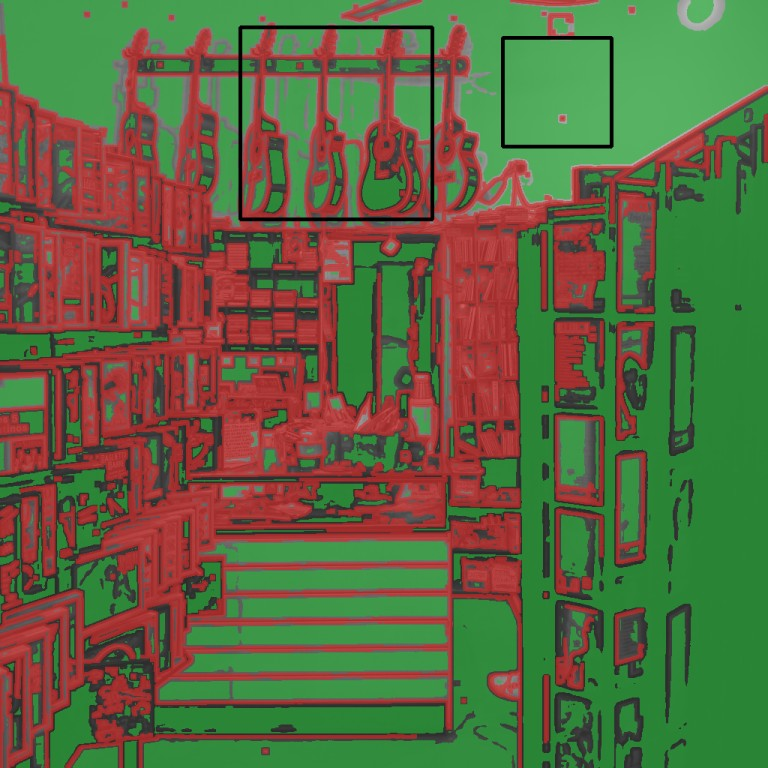
\includegraphics[width=\linewidth]{img/ejercicio_2/mascaras_regiones.jpg}
                \captionof{figure}{Máscaras y ROI.}
                \label{fig:ej2_mascaras}
            \end{minipage}\hfill
            \begin{minipage}[c]{0.70\linewidth} \centering \captionsetup{labelfont=bf}
            \begin{tblr}{
                cells={valign=m, halign=c, font=\small}, colspec={Q[l] Q Q Q Q},
                rowsep=0.8pt, colsep=4pt, hlines, vlines,
                row{1,2}={bg=gray!15, font=\small\bfseries},
                cell{1}{1}={r=2}{halign=c}, cell{1}{2}={c=2}{}, cell{1}{4}={c=2}{},
                cell{6}{2}={bg=gray!25}, cell{6}{3}={bg=gray!25}, cell{5}{4}={bg=gray!25}, cell{5}{5}={bg=gray!25} }
                Imagen & Bordes & & Homogéneas & \\
                & PSNR [dB] $\uparrow$ & SSIM $\uparrow$ & PSNR [dB] $\uparrow$ & SSIM $\uparrow$ \\
                Ruidosa & 20,55 & 0,610 & 21,18 & 0,123 \\
                Gaussiano $\sigma=2$ & 21,93 & 0,632 & 34,62 & 0,866 \\
                Gaussiano $\sigma=4$ & 19,78 & 0,412 & 34,75 & 0,899 \\
                Bilateral $(4, 100)$ & 26,34 & 0,812 & 34,59 & 0,831 \\
            \end{tblr}
            \captionof{table}{Métricas por región con las máscaras.}
            \label{tab:ej2_regiones}
            \end{minipage}
        \end{figure}

        En las zonas homogéneas las máscaras confirman lo observado en la ROI, ya que el gaussiano $\sigma=4$ supera al bilateral en SSIM (0,899 contra 0,831) con un PSNR similar, cercano a 34,6 dB. En los bordes, en cambio, la diferencia resulta mayor que en la ROI. El gaussiano $\sigma=4$ queda incluso por debajo de la imagen ruidosa (SSIM 0,412 contra 0,610), mientras que el bilateral llega a 0,812. En la ROI de borde el gaussiano parecía mejorar la imagen (SSIM de 0,322 a 0,658) porque la pared lisa que incluye el recorte compensaba los contornos que borronea.

    \subsection{Mapa de similitud estructural}

        La \textbf{Figura \ref{fig:ej2_ssim}} muestra el mapa SSIM local de la mejor y de la peor configuración (en rojo la similitud alta y en azul la baja). Con $(4, 100)$ casi toda la imagen queda por encima de 0,8 y la similitud sólo baja en las texturas finas, como los lomos de discos y los marcos de la izquierda. Con $(2, 20)$ el patrón se invierte, porque los contornos se conservan (rojo) pero las superficies planas siguen ruidosas (azul). Es decir, la peor configuración preserva los bordes, pero no cumple la función de suavizar.

        \begin{figure}[htbp] \centering
            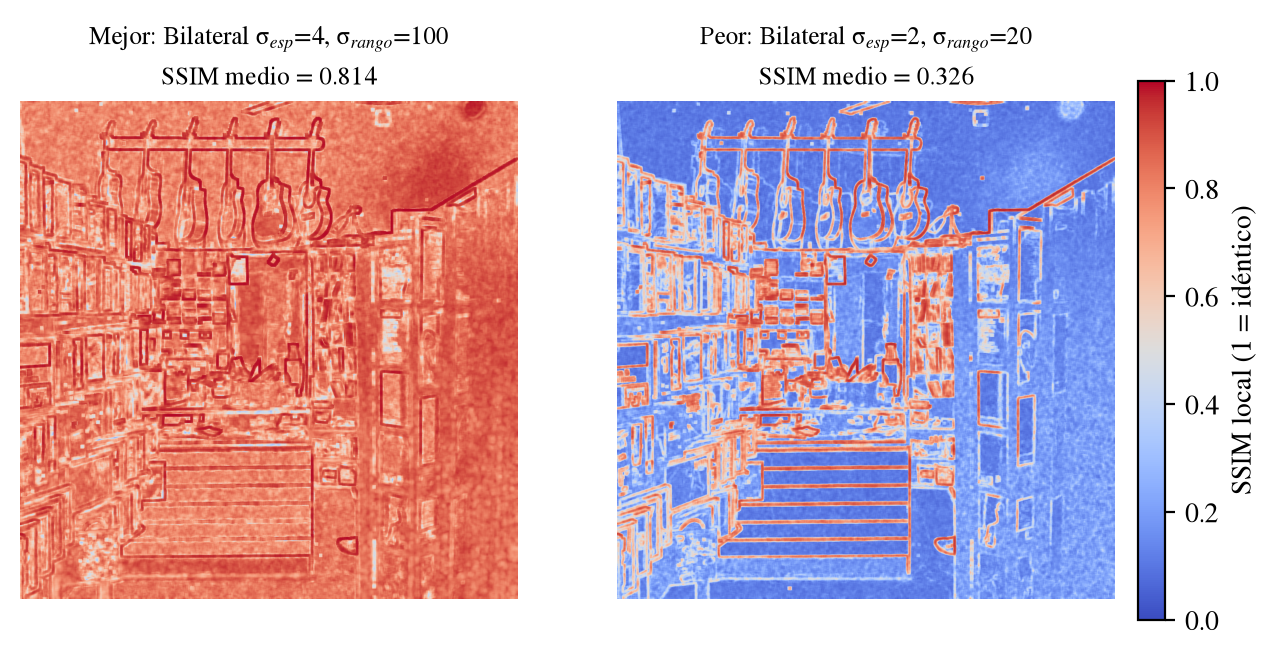
\includegraphics[width=0.64\linewidth]{img/ejercicio_2/mapa_ssim.png}
            \caption{Mapa SSIM local de la mejor (izquierda) y la peor configuración (derecha).}
            \label{fig:ej2_ssim}
        \end{figure}

    \subsection{Desempeño frente a los tipos de ruido más comunes}

        Se repitió el barrido con los cuatro ruidos típicos \cite{ej2:catedra} (\textbf{Figura \ref{fig:ej2_ruidos}}). El ruido \textbf{gaussiano} usa $\sigma=25$ y el de \textbf{sal y pimienta} afecta al 5 \% de los píxeles. El \textbf{aleatorio} se modeló como uniforme en $\pm43$ niveles, con la misma varianza que el gaussiano, y la \textbf{cuantificación} reduce cada canal a 8 niveles (3 bits). Para cada ruido se eligió la mejor configuración de cada familia por puesto promedio. La mediana se agregó sólo como referencia (\textbf{Tabla \ref{tab:ej2_ruidos}}).

        \begin{figure}[H] \centering
            \begin{subfigure}[t]{0.19\linewidth}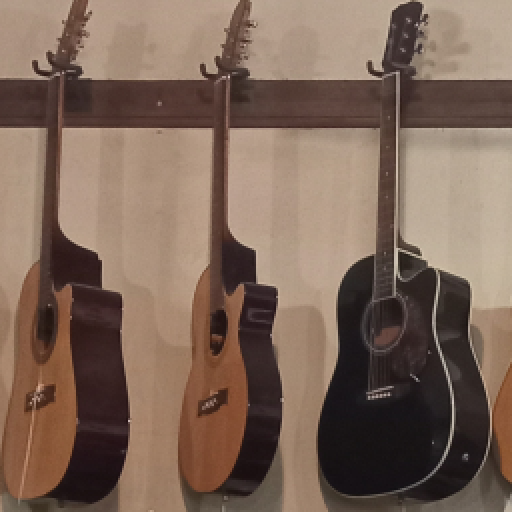
\includegraphics[width=\linewidth]{img/ejercicio_2/roi_borde_original.png}\caption{Referencia}\end{subfigure}\hfill
            \begin{subfigure}[t]{0.19\linewidth}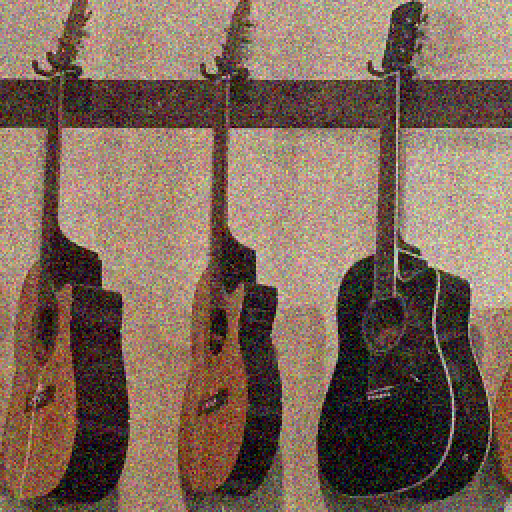
\includegraphics[width=\linewidth]{img/ejercicio_2/ruido_gauss.png}\caption{Gaussiano}\end{subfigure}\hfill
            \begin{subfigure}[t]{0.19\linewidth}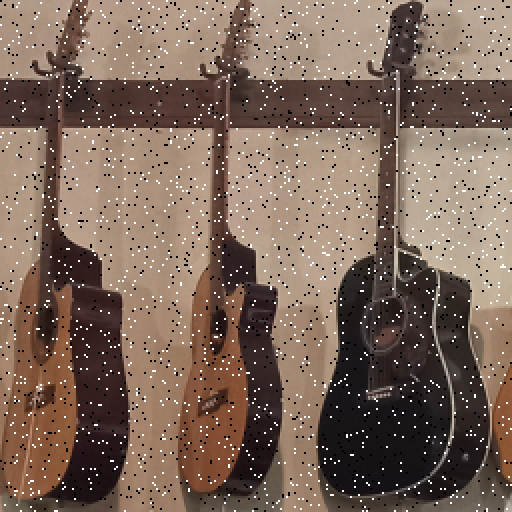
\includegraphics[width=\linewidth]{img/ejercicio_2/ruido_sp.png}\caption{Sal y pimienta}\end{subfigure}\hfill
            \begin{subfigure}[t]{0.19\linewidth}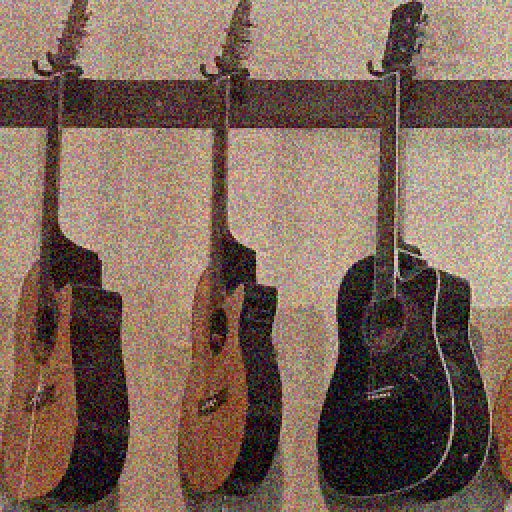
\includegraphics[width=\linewidth]{img/ejercicio_2/ruido_unif.png}\caption{Aleatorio}\end{subfigure}\hfill
            \begin{subfigure}[t]{0.19\linewidth}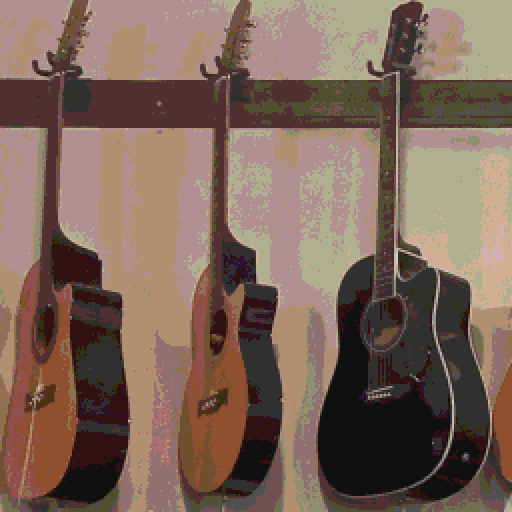
\includegraphics[width=\linewidth]{img/ejercicio_2/ruido_cuant.png}\caption{Cuantificación}\end{subfigure}
            \caption{ROI de borde de la referencia y de sus cuatro versiones contaminadas.}
            \label{fig:ej2_ruidos}
        \end{figure}

        \begin{table}[H] \centering \setstretch{1.05} \captionsetup{labelfont=bf}
            \begin{tblr}{
                cells={valign=m, halign=c, font=\small}, colspec={Q[l] Q Q Q Q},
                rowsep=0.8pt, colsep=5pt, hlines, vlines,
                row{1}={bg=gray!15, font=\small\bfseries},
                cell{2}{4}={bg=gray!25}, cell{3}{5}={bg=gray!25}, cell{4}{4}={bg=gray!25}, cell{5}{4}={bg=gray!25} }
                Ruido & Sin filtrar & Mejor gaussiano & Mejor bilateral & Mediana (ref.) \\
                Gaussiano      & 20,90 / 0,301 & 26,30 / 0,769 con $\sigma=2$ & 29,84 / 0,814 con $(4, 100)$ & 26,49 / 0,672 con $5\times5$ \\
                Sal y pimienta & 17,50 / 0,360 & 25,62 / 0,719 con $\sigma=2$ & 17,61 / 0,365 con $(2, 100)$ & 31,46 / 0,945 con $3\times3$ \\
                Aleatorio      & 20,84 / 0,297 & 26,27 / 0,766 con $\sigma=2$ & 29,55 / 0,795 con $(4, 100)$ & 25,73 / 0,590 con $5\times5$ \\
                Cuantificación & 29,30 / 0,843 & 25,96 / 0,787 con $\sigma=2$ & 31,19 / 0,904 con $(4, 50)$ & 27,41 / 0,813 con $3\times3$ \\
            \end{tblr}
            \caption{PSNR [dB] / SSIM por tipo de ruido. En gris, el mejor resultado de cada fila.}
            \label{tab:ej2_ruidos}
        \end{table}

        \begin{itemize}[label=\textbullet]
            \item \textbf{Gaussiano y aleatorio se comportan igual}. Ambos son de media cero e independientes entre píxeles, así que promediar los cancela, y el bilateral $(4, 100)$ gana en los dos casos.
            \item \textbf{Ante sal y pimienta el bilateral no hace nada} (17,61 contra 17,50 dB). Un píxel en 0 o 255 no tiene vecinos ``parecidos'', así que sólo se promedia consigo mismo. La mediana $3\times3$ es la indicada (SSIM 0,945).
            \item \textbf{En la cuantificación el bilateral mejora la imagen} (SSIM de 0,843 a 0,904). Los escalones de 32 niveles entre bandas quedan dentro de $\sigma_{rango}=50$, mientras que los bordes reales, mucho mayores, se preservan. El gaussiano, en cambio, la empeora.
        \end{itemize}

    \subsection{Preguntas y análisis}

        \begin{itemize}[leftmargin=*]
            \item \textbf{¿En qué regiones de la imagen se observan diferencias más notables entre el filtro gaussiano y el bilateral? Identificar zonas de borde y zonas homogéneas.}

                Las diferencias se concentran en los bordes, como los contornos de las guitarras, estantes, tablas del mostrador y textos, donde el gaussiano $\sigma=4$ baja el SSIM a 0,412 y el bilateral lo sube a 0,812. En las zonas homogéneas, como la pared o el frente del mostrador, ambos dejan la superficie lisa con un PSNR cercano a 34,6 dB, y el gaussiano queda apenas por delante en SSIM (0,899 contra 0,831).

            \item \textbf{Explicar conceptualmente cómo el filtro bilateral logra preservar bordes mientras suaviza. ¿Qué rol cumple cada uno de sus dos términos (espacial y rango)?}

                El término espacial $G_{\sigma_{esp}}$ define el alcance del promedio, igual que en el gaussiano, y el término de rango $G_{\sigma_{rango}}$ reduce el peso de los vecinos cuyo color difiere del píxel central. Junto a un borde, los vecinos del otro lado son muy distintos y reciben un peso casi nulo, por lo que el promedio mezcla sólo píxeles del mismo lado y suaviza dentro de cada región sin cruzar el contorno.

            \item \textbf{¿Qué ocurre cuando $\sigma_{rango}$ es muy pequeño? ¿Y cuándo es muy grande? ¿En qué caso el filtro bilateral se comporta similar a un filtro gaussiano estándar?}

                Si $\sigma_{rango}$ es menor que la diferencia que el propio ruido genera entre vecinos (unos 85 niveles en la distancia de color de OpenCV), ningún vecino se considera parecido y el ruido queda, y con 20 el SSIM no pasa de 0,357. Si es mucho mayor que el contraste de los bordes, el peso de rango vale casi 1 y el filtro se vuelve un gaussiano, y con $\sigma_{rango}=1000$ su salida coincide con la de un gaussiano de $13\times13$ con un PSNR de 43 dB entre ambas.

            \item \textbf{Comparar el costo computacional de ambos filtros. ¿El filtro bilateral es significativamente más lento? ¿Vale la pena el costo adicional según la aplicación?}

                Sí, el gaussiano tardó entre 4,8 y 17,3 ms por imagen y el bilateral entre 17,1 y 153,5 ms (la configuración elegida, 14 veces más que el mejor gaussiano), porque no es separable y recalcula sus pesos en cada píxel. Vale la pena cuando los bordes importan, como en medición, segmentación o fotografía, porque gana 0,045 de SSIM global y 0,18 en los bordes, mientras que en video en tiempo real de alta resolución, o si la etapa siguiente no usa bordes, alcanza con el gaussiano.

            \item \textbf{Describir un escenario real donde el filtro bilateral sería superior al gaussiano.}

                En la inspección óptica automatizada de placas impresas o de piezas mecanizadas con cámaras de bajo costo, el ruido del sensor genera falsos defectos y el gaussiano corre y ensancha los contornos de pistas y bordes que luego se miden. El bilateral limpia el ruido de las superficies y mantiene los contornos nítidos, de modo que la resta contra la plantilla y la medición dimensional siguen siendo precisas.
        \end{itemize}

    \subsection{Pipeline propuesto}

        La \textbf{Figura \ref{fig:ej2_pipeline}} resume el procedimiento. Parte de una referencia limpia, obtenida al reducir la foto original, y de su versión con ruido controlado. Después aplica las doce configuraciones de ambos filtros, las ordena por SSIM y PSNR y verifica el resultado por regiones, con el perfil y con el mapa SSIM. Por último, contrasta la elección frente a otros tipos de ruido antes de recomendarla.

        \begin{figure}[htbp] \centering
            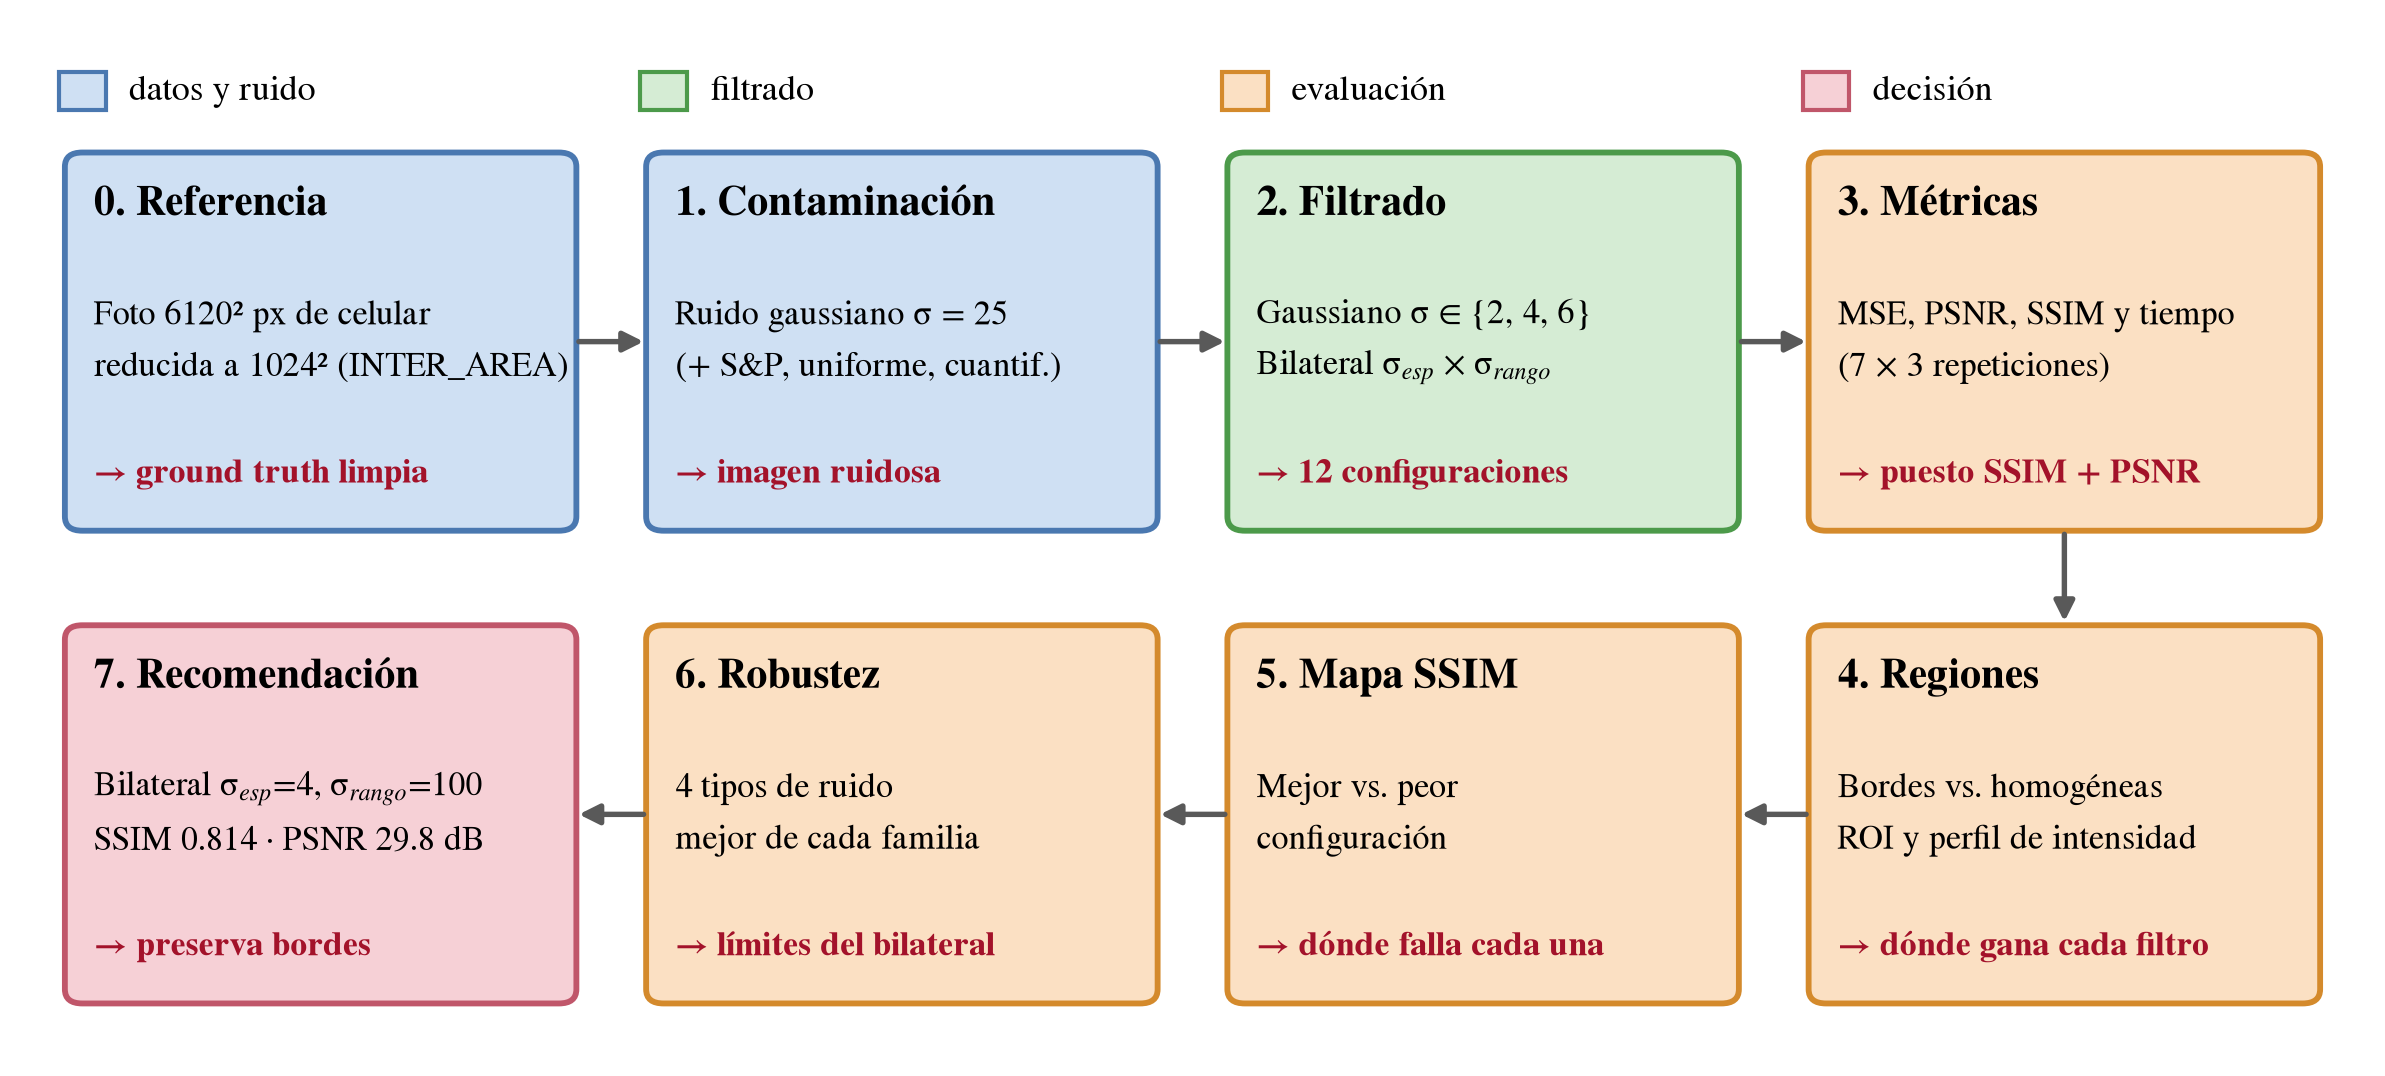
\includegraphics[width=0.70\linewidth]{img/ejercicio_2/pipeline.png}
            \caption{Pipeline propuesto para comparar los filtros gaussiano y bilateral.}
            \label{fig:ej2_pipeline}
        \end{figure}

    \subsection{Conclusiones}

        Para esta imagen con ruido de $\sigma=25$ se recomienda el \textbf{filtro bilateral con $\sigma_{esp}=4$ y $\sigma_{rango}=100$}. Obtuvo el mejor SSIM (0,814) y puesto promedio, con 29,84 dB de PSNR, frente a 0,769 y 26,30 dB del mejor gaussiano. La observación coincide con las métricas, ya que el bilateral conserva el contorno de las guitarras, los estantes y los textos (\textbf{Figuras \ref{fig:ej2_rois} y \ref{fig:ej2_perfil}}), mientras que el gaussiano sólo alcanza un resultado aceptable con $\sigma=2$, que en los bordes apenas supera a la imagen ruidosa (SSIM 0,632 contra 0,610, \textbf{Tabla \ref{tab:ej2_regiones}}), y con $\sigma=4$ o $6$ borronea la escena. Las dos métricas divergen sólo en $(2, 100)$, que el PSNR preferiría aunque deja más ruido residual en las zonas lisas (\textbf{Figura \ref{fig:ej2_grano}}), y el SSIM corrige esa elección.

        El parámetro clave es $\sigma_{rango}$, que tiene que superar la diferencia que el ruido produce entre vecinos y quedar por debajo del contraste de los bordes. Como OpenCV a color la mide sumando los tres canales, los valores útiles son mayores que en escala de grises. El bilateral no sirve para ruido impulsivo, donde corresponde la mediana, pero sí atenúa el bandeo de la cuantificación.

        Para un pipeline automatizado, lo planteable es justamente combinar el bilateral $(4, 100)$ como filtro con el puesto promedio entre SSIM y PSNR como criterio de selección, ya que una sola métrica puede llevar a configuraciones visualmente peores. Como requiere una referencia limpia, una posible solución en imágenes reales sin \textit{ground truth} los parámetros podrían calibrarse con la pérdida autosupervisada.
